\documentclass[a4paper]{article}

\usepackage[latin1]{inputenc}
\usepackage{palatino}
\usepackage[usenames]{color}

\usepackage{hyperref}

\usepackage{chngpage}
\usepackage{graphicx}

\usepackage{booktabs}
\usepackage{multirow}

\usepackage[]{algorithm2e}
\usepackage{varwidth}

\usepackage{setspace}
\usepackage{hyperref}


\usepackage[babel, en, nat, farve, titelside]{ku-forside}

% nbuf command
\newcommand{\nbuf}{\textit{nbuf} }

\usepackage{fancyhdr}
\pagestyle{fancy}
\lhead{Asbj\o rn Thegler}
\chead{Master's Thesis}
\rhead{October 2015}

\renewcommand{\headrulewidth}{0.4pt}
\renewcommand{\footrulewidth}{0.4pt}
\setlength{\belowcaptionskip}{-10pt}

%% a point to check
\definecolor{checkcolor}{rgb}{0.75, 0.75, 0.75}
\newsavebox{\definitionbox}
\newenvironment{checkit}{%
\begin{lrbox}{\definitionbox}
\begin{minipage}[t]{0.85\textwidth}%
}%
{\end{minipage}\end{lrbox}%
\begin{center}{\colorbox{checkcolor}{\usebox{\definitionbox}}}%
\end{center}}

\opgave{Master's Thesis}
\title{Automatic $n$-buffering for Big Data processing}
\undertitel{Department of Computer Science}
\author{Asbj\o rn Thegler - asbjoern@gmail.com}
\date{October 2015}
\vejleder{Professor Brian Vinter}


\begin{document}

\maketitle

\sloppy

\pagenumbering{roman}
\begin{abstract}
\begin{doublespace}
This study attempts to construct a generally applicable library for efficient and parallel processing of data from generic data streams.

The \nbuf library is intended to be used mainly for live processing of very voracious streams. This is useful when huge amounts of data is being generated and when processing those data must be done before archiving them in slow storage solutions.

The library has been built with the abstract synchronization primitives made available in C++11, which is based on POSIX threads. Further care was placed in making the library as flexible as possible for every thinkable scenario.

Benchmarking results shows that the library can fully utilize the rate of a data stream, when sufficient computational powers are available. In cases where there are additional constraints on the level of parallelism, the library exhibit brilliant latency hiding capabilities.

The library successfully enables developers to efficiently process streams of data in a concurrent manner, without extensive knowledge about multiprocessing and inter-process communication.\\

The \nbuf library can be found at \url{http://github.com/ath88/nbuf}. The current version is tagged as \textit{v0.1}.

\end{doublespace}
\end{abstract}

\newpage
\tableofcontents

\newpage
\pagenumbering{arabic}
\section{Introduction}
Big Data has become a huge topic over the last few years. Google Trends reveal that the interest for 'big data' has exploded since 2012. Huge companies worldwide speculate on how to profit from this new trend, and many widely respected conferences include entire tracks on how to work with Big Data.\\

There are many definitions to what Big Data really is. In 2001, an analyst from Gartner, Doug Laney, defined big data to consist of 3 V's\cite{3vs}. He defines them as \textbf{Velocity}, \textbf{Volume} and \textbf{Variety}.\\

\textbf{Velocity} refers to the speed at which data is produced. Previously, most data streams could be stored and analysed with primitive mechanisms, without much thought into architecture and algorithms. With the new velocity of data generation, it is necessary to design solutions that can handle and utilize very fast streams of information.

\textbf{Volume} refers to the huge volumes of data that are being gathered in recent times. Modern scientific equipment will generate several terabytes per day, which all have to be processed and stored. To support these growing amounts of data, it is necessary to keep producing larger and cheaper storage solutions.

\textbf{Variety} refers to the endless amounts of different formats that data is stored in. To be able to interpret such unstructured data, it is necessary to have a wide array of tools and mechanisms to analyse these different sorts of information.\\

In 2014, Mark van Rijmenam from Datafloq\cite{7vs} argued that the definition of Big Data could be extended with 4 additional V's. He defines them as \textbf{Veracity}, \textbf{Variability}, \textbf{Visualisation} and \textbf{Value}\\

\textbf{Veracity} refers to the validity of the data. Even though data is being generated, they are worthless if they are not correct. Smaller amounts of data can be sanity-checked manually, but these huge amounts of data cannot be checked for errors in any sensible way. The data generation mechanisms must be precise and correct.

\textbf{Variability} refers to the changing meaning of a subject. Languages and meanings change over time, and as such, the interpretation of data must adhere to the current context, and not a context that has been established over many years.

\textbf{Visualization} refers to the need for presenting the results from analysing Big Data in a sensible way. Two dimensional graphs can no longer express the multitude of findings that can be found in such huge datasets. New mechanisms will have to be created, which can be used to visualize interesting parts, such that decisions can be made on an informed basis.

\textbf{Value} refers to the potentially lucrativeness of the Big Data industry. While utilizing huge sets of information about customers can increase profit for many companies, these techniques are not cheap to use. Done wrong, a Big Data venture can cost a lot in storage and processing power.\\


This project does not aim to solve all problems encountered in the field of Big Data. The main focus of this study is to attempt to mitigate some of the difficulties that arise from having data streams with \textit{extreme velocity}. It will be done by creating a  library that uses several buffers to swap around, often referred to as \textit{Triple Buffering}.


\subsection{Terminology}
The first well known occurrences of the term \textit{Triple Buffering} stems from the computer graphics industry\cite{3buf}. This is a technique where the graphics card renders images into three different buffers. \textit{Triple Buffering} is a solution to a problem with the \textit{Double Buffering} technique. In this, a two buffers are used; a \textit{front-buffer} and a \textit{back-buffer}. 

In \textit{Double Buffering}, the card renders a frame into the back buffer, and the buffers swaps to allow the screen to show the picture from the front buffer. Since no synchronization exists between the card and the screen, a buffer swap can happen as the screen is reading from the front buffer, resulting in what is known as \textit{screen tearing} where the screen shows two different frames at once. An attempt to fix this problem is know as \textit{vertical sync}. This includes adding artificial delays to the cards renderer, to match the frame rate of the consuming screen, effectively slowing down the graphics card.

To better solve this problem, a third buffer is employed, effectively making it \textit{Triple Buffering} rather than \textit{Double Buffering}. The card can now switch between two back-buffers, and always have a free buffer to write a new frame to. If the screen is too slow, frames will simply be lost, with no greater loss to the viewer. This extra buffer obviously require extra memory, but modern graphics cards have plenty of memory.\\


\subsection{Triple Buffering Big Data}
\textit{Triple Buffering} within computer graphics is a different concept than \textit{Triple Buffering} within data processing. There are many similarities, however, and we can translate parts of the solution to increase data processing capabilities. The bottlenecks of a graphics card are namely the rate at which the graphics card can render images, and the rate at which the screen can show those images. If the screen has a low frame rate, then a very fast graphics card is useless, and vice versa. 

This translates to the I/O problems we encounter when working with data processing. If we cannot process and store data at the same velocity they are being generated in, then we have to throw some data away, or slow down the data generator. The computer graphics industry increased throughput by utilizing more space, by adding an extra buffer. This concept can solve, or at least mitigate, some of the I/O problems related to processing data at high velocity.\\

The focus of this study is to produce a library that enables programmers to process or transform large amounts of data in an efficient and concurrent way, without having to worry about concurrency issues and memory management. The library should be generic, such that it is as generally applicable as possible, while still being useful and simple enough to understand for people who aren't familiar with multiprogramming. It is important to note that this project in no way introduces new technology or uncovers scientific ground. This is a study in combining existing technology and knowledge to create a highly optimized and effective library.


\subsection{Motivation}
This study did not manifest from thin air. Many people have contemplated building such a library. \textit{Triple Buffering} has been used many places, many times before, and it is a well-known technique. The reason why this project was undertaken now, and not 10 years ago or in 10 years, is a combination and collision between Moore's Law, data bus speed and the growing Open Source community, both within academia, but also within established industries. 

Having a library that exerts these capabilities, that can be scrutinized and improved by everyone, will help organizations all over the world when they will have to process fast data streams.\\

There are some existing solutions to this problem already. The Apache Foundation has both \textit{Apache Hadoop}\footnote{Apache Hadoop, \url{https://hadoop.apache.org/}} and \textit{Apache Storm}\footnote{Apache Storm, \url{http://storm.apache.org/}}, which both deploy a distributed map-reduce cluster. This project will separate itself from these solutions by being an library rather than a service. It will require a programmer to include the library in software, rather than configuring a distributed cluster.


\subsubsection{The I/O Problem}
Moving data to and from computational resources inherently results in I/O operations. Depending on the transfer rate of the data storage, these operations quickly becomes a bottleneck for the entire process. If we then proceed to not extract data from these streams at all time, then a lot of time time is spent on waiting. In reality, the process could pre-load data during processing and reduce the time spent on waiting for I/O. To process data as fast as possible, we want to fully utilize the I/O resource. 

When processing data, the traditional method consists of the following steps;

\begin{enumerate}
\item Load data into buffer from source
\item Process or transform data
\item Write data to destination
\item If there is more data; go to step 1
\end{enumerate}

If the computational task of processing or transforming the data is very large, the I/O becomes negligible. In this case, most time is spent on step 2, and interlacing the I/O operations not give a significant improvement. Parallelizing step 2, however, will allow for very significant improvements. This will include adding more workers that can process the data in parallel.

If the computational task of processing or transforming the data is very small, most of the execution time will be spent waiting for I/O. An example could be a simple copy of a file from one disk to another. In this case, there are two I/O resources, which are being used in step 1 and step 3, namely the \textit{input stream} and the \textit{output stream}. This means that only one of the resources are being used at any given moment. To improve this mechanism, we could have two concurrent workers, each occupying one resource, to utilize both of the resources at any given time. In case of a computational task, a third worker could then perform step 2, which is exactly how \textit{Triple Buffering} works.\\

This study will focus on the case where neither the execution, nor the I/O operations are negligible. In this case, it is important to be able to be able to parallelize step 2, while having additional workers occupying the I/O resources at all times. The library will be most useful in these cases, but will also be applicable in other cases.


\subsubsection{The Generic Problem}
When programmers develop software, they are generally encouraged to utilize established libraries whenever possible, instead of relying on their own ability to create both complex and correct code. Often, a programmer encounters a specific problem, that can be translated into a general problem which has already been solved multiple times. The productivity of the programmer can increase greatly, when using tested and accomplished libraries. 

Some topics are inherently difficult for programmers, such as memory management and concurrency, often leading to memory leaks and race conditions. When utilizing widely used and established libraries, these problems are often already addressed by many other programmers.\\

Within the Open Source community, it is common practice to make ones code available for others to use. In theory, when many organizations use the same tool or library, errors are found, reported and corrected much faster than when code is only used privately or within a single organization. Over time, this often result in libraries that are used globally, and has many contributors. This is known as crowd-sourcing.\\

When a general library that solves a general problem does not exist, programmers must write custom code that solves the problem. This will result in many programmers solving their specific problem over and over again. They cannot share their solutions, because they have all solved their own specific problem, and every problem has slight differences. At some point, a programmer will realize that there is a pattern and pick up the task to attempt to build a generally applicable library.\\

When a problem is simple, using a complex library might be too much work, since many libraries has a ton of options that might be irrelevant to the task at hand. Reading the manual of many tool can be a daunting task, while often simple problems can be solved faster with custom code. Attempting to identify what library might fit the current problem can be a sizeable project in itself. 

Open Source projects tend to have organic growth. Without tight steering from some small group of committed programmers, a project will be monolithic and it will suffer from \textit{software bloat}. A tool or a library is usually created to solve a problem. Over time, the problem-body might be extended to include more features. In these cases, many people using the tool or library does not need the newer features, and to them, the features are merely an annoyance. In 1996, Jamie Zawinski wrote the following about \textit{software bloat}\cite{bloat}:

\begin{quotation}
  Every program attempts to expand until it can read mail. Those programs which cannot so expand are replaced by ones which can.
  -- Jamie Zawinski, 1996
\end{quotation}

This is clearly put very comically, but the reality is that this often happens. Software develops until it becomes to slow and cumbersome. At this point, it is replaced by new and lean software, which overtime grows until it becomes almost identical to the software it replaced. To avoid this tendency, it is important to keep a very strict process, when deciding what features to include.
    

\subsubsection{Use Cases}
The library that is built over the course of this study could be used for several purposes. Large amounts of data are being processed in many places. Following are some use cases where using such a library could be a good solution.\\

Modern hash algorithms are designed to ensure the integrity of a collection of data. As an example, when large files are transported from one place to another, it is important to ensure that the data is intact upon arrival. A hash-value can be calculated before and after transport, to be compared afterwards. In this case, the tool used for transmitting the data could use a buffering mechanism, which calculates the hash value, as it is read from disk, and as it is written to disk. This would be far more efficient, than to read the file from disk after transport, only to calculate the hash-value. The data is already passing through memory on both sides of the transportation, and utilizing the data here would be beneficial.\\

Additionally, the command line tools \textit{md5sum} and \textit{sha512sum} both have implementations that read 512 bytes at a time, which results in many I/O operations, in case of large files. Many of those operations could be avoided, if more memory is available for multiple larger buffers. Further, using a concurrent approach to this problem, could introduce some latency hiding, which will improve the runtime of the tools.\\

When large amounts of sensor data are received via a network, they are usually written directly to disk, before they get processed. In cases where much of the data is merely noise it could be good to have an option to process the data as it arrives, instead of delaying until after is has been written to disk. This can include gathering statistics, calculating hash values or filtering irrelevant data. An example could be a network of rain water gauges. When there is no rain, it is unnecessary to store the information.\\

The \textit{ESS project}\footnote{European Spallation Source, \url{https://europeanspallationsource.se}.}  aims to create a state of the art super microscope. Such microscope is bound to produce tons of information, which many different peers will be interested in analysing. The raw data will have to be stored, for situations where questions arise about data integrity. Typically, the data will be stored on inexpensive tape or cheap hard disks, which are very slow storage solutions. 

Whenever data is generated from the microscope, there will be a set of different  statistical results which will always be interesting. If these statistics could be gathered as the data is in-route to the storage solution, it would not be necessary to load the data back into memory to perform these statistical calculations. This would save a lot of waiting time and free up time to perform other tasks.


\newpage
\section{Theory and Analysis}
This section will explain the ideas and concepts that are applied during the design and implementation of the \nbuf library. 

The first section will explain how concurrency is handled and how correctness is ensured. This also entails how to ensure that the library will always terminate when used correctly. 

The second section will explain how the study handles aspects related to data, I/O and how to handle the enormous amounts of data, and how different data streams affect the resulting library.

The third section will reason on what technical results can be expected from this study. This will mainly focus on benchmarking, and how different configurations can affect the measured results.



\subsection{Concurrency}
Concurrency has proven to be hard for the human mind to understand, design and work with. When done wrong, software can easily
include deadlocks or other race conditions. This section will explain some of the pitfalls of concurrency and how to avoid them.


\subsubsection{Flow and Deadlocks}
Concurrency done wrong can result in processes spinning out of control, or not running at all. The widest known example used in teaching about deadlocks is known as the Dining Philosophers Problem, which was presented by E. W. Dijkstra in 1971. [Dijkstra, Hierarchical ordering of sequential processes]

Deadlocks and deadlock prevention is paramount when working with concurrency, but explaining why should be trivial at this point. I will suggest reading Concurrent Systems, by Jean Bacon [reference!], if you want to learn more on this topic. When working with concurrency, it is important to have knowledge of how deadlocks can happen, and what measures can be deployed to avoid them, both theoretical and practical.


\subsubsection{Finite-state Diagrams}
Any process can be interpreted as a finite-state machine. Doing so will help understand the process, its possible states, and the triggers that will change the internal state of the process. This is known as the scientific body of "Automata Theory" and what I will elaborate on here, is a subset of this field.

To gain a better understanding of a finite-state machine, a finite-state diagram can be created. It is a tool that can be used to ensure that the process at hand reacts and interacts as expected. Finite-state diagrams are trivial to both create and understand, and can be used to reason about a process, as a development tool and as documentation about a certain system or process. It gives an abstract idea of how a concrete process progresses.\\

% State Diagram 1
\begin{figure}
	\begin{adjustwidth}{-0.5in}{-0.5in}
    \centering
    \def\svgwidth{\columnwidth}
    \input{figures/door.pdf_tex}
  	\caption{This is an example of a finite-state diagram. It represents a door which can be in 3 states, and there are 4 different transitions.}
	\label{figure:door}
	\end{adjustwidth}
\end{figure}

In figure \autoref{figure:door} there is an example finite state diagram. This diagram is quite simple, and shows how a door with a lock will behave.

There are 3 states, \textit{Open}, \textit{Closed} and \textit{Locked}. The process must be in either state at any one time. Further, there are 4 different events that can happen, \textit{open}, \textit{close}, \textit{lock} and \textit{unlock}. These can happen at any time, and the door will transition to another state. There are implicit transitions on every state, which lead to itself on events that there are not explicit transitions for. For example, locking an open door will make the door transition to the same state, while locking a closed door will make the door transition to the \textit{Locked}-state.\\

When explaining how the \nbuf framework works, I will use finite-state diagrams to show how the worker threads behaves. This helps understand how the threads are initialized, used and terminated, and more importantly, how they interact with each other through synchronization primitives.


\subsubsection{Synchronization Primitives}
Concurrent programming entails using some kind of multiprocessing. This is usually done by using multiple threads which can be scheduled individually on cores. This allows multiple thread to run simultaneous, using the same memory space. While sharing memory is very practical, it also brings several pitfalls that can seem in-obvious to a programmer who aren't used to concurrency. To solve these problems, it is necessary to use some kind of synchronization, to ensure \textit{thread-safety}.

All synchronization mechanisms are based on the hardware instruction \textit{test-and-set}. Using this instruction, locks, semaphores and queues can be implemented. These are all known as \textit{Synchronization Primitives}. These are abstractions, and are intended to make it easier to make more elaborate synchronization in systems. The primitives that are relevant to this project are the following:

\begin{itemize}
\item \textbf{Mutex} - A mutex is merely an advanced locking primitive. The name is derived from 'mutual exclusion'.
\item \textbf{Condition Variable} - A condition variable is a primitive that can be used to make threads wait for specific events.
\item \textbf{Future} - A future is a primitive that encapsulates the result of an asynchronous calculation for the calling thread. The naming is intended to be understood as; \textit{In the future I have this}.
\item \textbf{Promise} - A promise is a primitive that encapsulates the result of an asynchronous calculation for the executing thread. The naming is intended to be understood as; \textit{I will have to fulfil the promise}.
\end{itemize}


A \textbf{mutex} is basically a lock. It can be used to protect critical section of code. It is a higher-level construct, and automatically makes a thread wait, when it attempts to obtain the mutex while it is already taken.\\

A \textbf{Condition Variable} is a primitive which can be used to block threads on purpose. A thread can be set to wait on a specific condition variable, which means that it will block until another thread has notified one or all threads that are waiting on that specific condition variable. Most condition variables have a mechanism for notifying just one thread, or all threads. This is practical, since there might be cases where many threads are waiting, but only one can continue, and the other threads will have to wait for some time. In other cases, all threads might be able to continue working after this event. 

Normally, using a condition variable requires that some condition has to be true, before continuing, since many implementations allow threads to wake up spuriously, even though no threads has notified. In case of a spurious wakeup, the thread should be able to detect if the wakeup was due to a notification, or if it was spurious.\\

A \textbf{Future} is a primitive which is created by the calling thread, sometimes referred to as the master thread. This thread creates the future primitive and pairs it with a task that can be performed asynchronously. The task can be started, and the master thread can perform other calculations. When the master thread needs the result from the task, it can wait for the future to be finished, such that the result can be retrieved from the future.\\

A \textbf{Promise} is a primitive which is created by the calling thread, and passed off to another thread. From the promise, the calling thread can create a future. The worker thread which received the promise as a parameter can set the content of the promise when it exits, such that it can be retrieved.\\

When working with multiple threads, it is historically very hard to handle exceptions that happens in other threads than the master thread. When a thread encountered an exception, it would terminate, and throw away the exception. A solution was to define a shared exception variable prior to starting the task, which could then be used to inform about what happened to the thread. 

When using the Future-Promise constructs, exceptions are stored in the promise and re-thrown when the master thread attempts to retrieve the result through the future. This makes debugging concurrency a lot easier, since the exceptions are no longer thrown away, and doesn't require the programmer to declare exception variables before every asynchronous call.


\newpage
\subsection{Data Handling}
Working efficiently with data is no small task. There are many physical limits to what results we can obtain, but getting to these limits often requires a lot of thought, since there are many abstraction layers between hardware and software. This section will elaborate on how to work with these sizes of data in a correct and efficient manner.


\subsubsection{Data Marshalling}
When receiving and sending data to and from a stream, care should be taken when interpreting the data. The act of turning an object into a string representation is known as \textit{marshalling} or \textit{serialization}. The opposite act, turning a string representation into an object is called \textit{demarshalling} or \textit{de-serialization}.\\

There are many ways to serialize an object, depending on what data the object contains. If the object contains variable length strings, there are several ways to design the string representation. One solution is to decide on the maximum length of the string, and then allocate that same size in the string representation. This can result in a lot of unnecessary white space, if the string turns out to always be very small, compared to the allocated size. De-marshalling becomes trivial, because you know exactly where and how long the string is. Also, the size of the string representation can be predicted precisely.\\

Another solution is to use some kind of delimiters. Depending on the content of the string, we can use a symbol such as the pipe or a simple semi-colon. This solution saves a lot of space, but makes parsing harder, since it is necessary to inspect the data, before parsing it. Further, you cannot reason about the maximum size of the string representation, since the strings can have arbitrary length.\\

When using a very simple object structure, it may be easier to simply use the binary representation of the object. In some cases this will work, and others it will not. Different platforms and compilers may differ in how the memory layout of an object is constructed. This will lead to inconsistencies and ultimately in-correctness.\\

Google has given a solution to the marshalling problem with a mechanism they call Protocol Buffers \footnote{reference google project page}. They allow you to specify a data structure in a platform- and language-independent way, and have constructed cross-platform libraries for C++, Java and Python. These libraries can be used to create a protocol buffer object, from the specified structure. When desired, one such object can be marshalled, and de-marshalled by another program, on another platform or in another language. This helps keeping a consistent view of how data is interpreted and altered across multiple systems and implementations.

The Protocol Buffer implementations inspect the string representation when de-marshalling the data, and it is impossible to predict the length of an objects string representation, unless you yourself enforce fixed width-strings. While inspecting is slower than parsing a fixed-width string representation, Google has promised that the implementations are highly optimized. Further, they recommend keeping protocol buffer objects smaller than 1 megabyte.\\

When a developer uses the \nbuf framework, it is recommended to use a protocol buffer, when processing the data. However, since the \nbuf framework only allows fixed-width parsing, care must be taken to ensure that the width of the string representation is constant, or ensure that proper padding is added.


\subsubsection{Optimal Buffer Size}
Buffers are used everywhere. The optimal size is a ubiquitous definition, and all depends on what you want to \textit{optimize for}. In some cases, you want speed, in other cases, you want a low memory footprint.\\

Typically, you want the system to perform well, within some given constraints. Sometimes using too large buffers merely slows down a system, since other processes won't be able to allocate the desired memory.\\

When processing data, a buffer that is larger than the amount of data it needs to buffer is unnecessary. As an example, a video-buffer is large enough to ensure that connection fallouts of a certain size can be mitigated. If the buffer is so large that it can contain the entire video file, most of the buffer is wasted, since memory could easily be reused, when playing the video.\\

When using the \nbuf framework, using buffers that allows a single thread to contain the entire file in its local buffer, will make the framework behave inherently sequential. This reduces the multiprocessing capabilities of the framework. However, using too small buffers will induce extra overhead, since the amount of I/O operations will be increasing. Finding the right balance is essential, but it is hard to generalize what size will fit most projects.


\subsubsection{System Data Steams}
The \nbuf framework seeks to give an agnostic approach to how the streams behave. The framework should give the same results, when given the same data, whether the data comes from a network stream, a file stream, or a stream from a memory location. This means that it has to use only slightly abstract methods, on the streams that are supplied.\\

It is important to know how different streams behave, even though the framework must have agnostic behaviour. When benchmarking, it is indeed important, to be able to identify where and why certain results are attained.\\

In C++11, there are two different kinds of basic streams, which both inherit from a general stream type. These streams are known as \textit{string streams} and \textit{file streams}. A third kind of stream can be gained from third-party libraries, such as the Boost.Asio library\footnote{ http://www.boost.org/doc/libs/1\_59\_0/doc/html/boost\_asio.html}, namely a \textit{network stream}.\\

These three kinds of streams can be used in the \nbuf framework, which gives a very versatile system. Each kind of stream, however, has limitations which in general will limit the throughput of the framework.\\

A \textit{network stream} used as input is limited by the bandwidth of the connection to the data source. If the data source is on a local wired network, it is common to have a large bandwidth, while a remote data source, transmitting via a modem will have a drastically reduced bandwidth. The same limit applies when sending data to a network stream. However, most operating systems keep a buffer, such that the program can quickly return, while data may not be sent yet. The data may stay in the buffer for some time, until the operating system decides to transmit the data. If large amounts of data is transmitted at once, the buffer might be too small, and the operating system is forced to transmit some data, before returning control to the calling process.\\

A \textit{file stream} used as an input stream is limited by the bandwidth of the disk and the bus that connects the disk to the system. When traditional hard disks or tapes are used, locating data can be a slow task, and benchmarking such tasks will result in very inconsistent results. The disk has to seek to the right disk and location, before it is able to read the file. Newer technology, such as a solid state disk or raid configurations can mitigate or eliminate these inconsistencies. When a file stream is used as output, the operating system again buffers the data, which allows the calling program to return rather quickly. Similarly, with output data that is too large to fit in the buffer, the operating system will have to save some data to disk, before returning to the calling process.\\

A \textit{string stream} is a stream that streams directly from data that is already located in main memory. The bandwidth of such stream is only limited by the transfer rate of the main memory technology and the bus that connects the memory to the CPU. This is, without doubt, the fastest stream that can be used in the framework. When used as an output stream, it has the same fast transfer rate. The downside to this kind of stream is that it is very impractical, since you will hardly ever be able to fit all your data into a string stream, and if you do, you might as well have processed directly from the other stream, instead of putting data into the string stream.\\

When benchmarking the \nbuf system, we want to ensure that optimal I/O has been achieved. If the framework can handle concurrency from fast streams, slower streams should be trivial to handle concurrently.


\subsection{Theoretical Speed-up with Threads}
Most modern CPUs include multiple cores with hyper threading. On a single-core systems, only one thread can execute at any one time. On multi core systems, multiple threads can execute in parallel. If every process only contains a single thread, no memory is shared between multiple threads, unless explicit process memory sharing is used.\\

If a process contains several threads, the process can have several threads executing simultaneous on multiple cores. When tasks can be done in parallel, the entire bunch of tasks can be finished faster than if they were performed in sequence.\\

The \nbuf framework allows developers to interlace the tasks of \textit{reading}, \textit{processing} and \textit{writing} data. Following are a few examples of how the three tasks at hand can be interlaced.\\

In \autoref{figure:timings1} is an example of how the framework could interlace if both the read-, the process- and the write-task took an identical amount of time. In this case, three threads would be able to completely occupy both the read and the write resource at all times. If another thread was added, it would only introduce idle times, while waiting for the resources to become available.\\

% Timings 1
\begin{figure}
	\begin{adjustwidth}{-0.5in}{-0.5in}
    \centering
     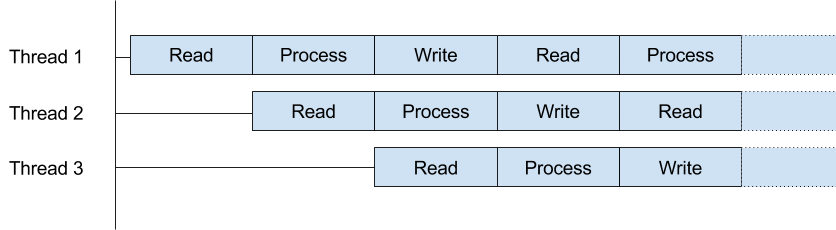
\includegraphics[scale=0.5]{figures/timings1.png}
  	\caption{This is an example of how the \nbuf framework could interlace, if all three tasks are similar in time taken.}
	\label{figure:timings1}
	\end{adjustwidth}
\end{figure}

% Timings 2
\begin{figure}
	\begin{adjustwidth}{-0.5in}{-0.5in}
    \centering
     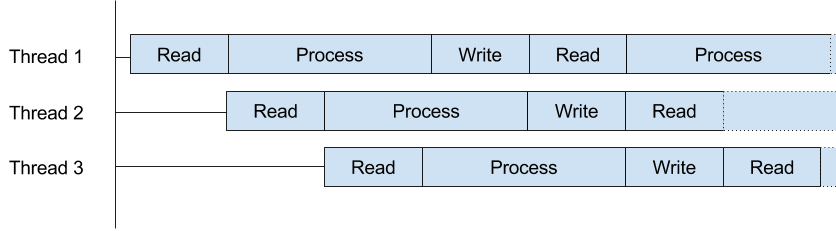
\includegraphics[scale=0.5]{figures/timings2.png}
  	\caption{This is an example of how the \nbuf framework could interlace, if the processing task takes more time than the read and write tasks.}
	\label{figure:timings2}
	\end{adjustwidth}
\end{figure}

In \autoref{figure:timings2} is an example of how the framework could interlace if the processing task takes longer time than the read and the write task. The processing task can be done in parallel, but after the third thread has read, the read-resource is available for some time, until the first thread is done processing and writing. In this case, more threads are needed to fully utilize the read- and write-resources.\\


In \autoref{figure:timings3} is an example of how the framewould could interlace if the processing task takes less time than the read and the write task. The read- and write-resources are occupied at all time, but threads are merely waiting idle, for resources to become available. In this case, two threads would not be able to fully utilize the read- and write-resources, but the smaller the processing task becomes, the more idle time there will be. In the case where there is no processing at all, only two threads would be able to fully utilize the resources. \\

% Timings 3
\begin{figure}
	\begin{adjustwidth}{-0.5in}{-0.5in}
    \centering
     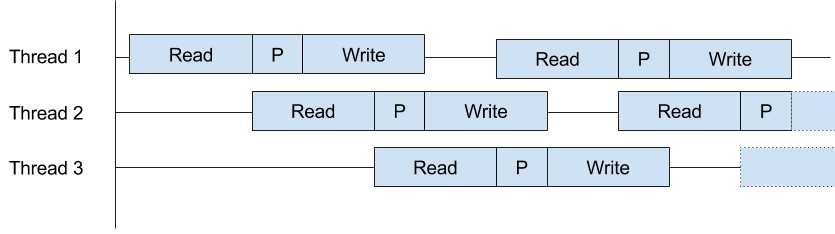
\includegraphics[scale=0.5]{figures/timings3.png}
  	\caption{This is an example of how the \nbuf framework could interlace, if the processing task takes less time than the read and write tasks.}
	\label{figure:timings3}
	\end{adjustwidth}
\end{figure}

In \autoref{figure:timings4} is an example of how the framework could interlace if the processing task takes more time than the read and the write task, and the processing step can only be done sequentially. The read- and write-resources are not fully utilized, but processing happens as often as possible. Adding or removing threads would not increase the utilization of the read- and write-resources, so in this case, the utilization cannot become any higher.\\

% Timings 4
\begin{figure}
	\begin{adjustwidth}{-0.5in}{-0.5in}
    \centering
     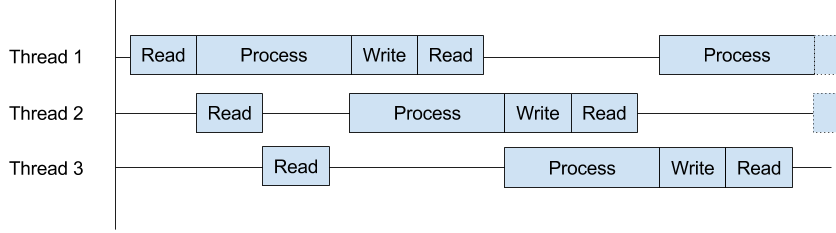
\includegraphics[scale=0.5]{figures/timings4.png}
  	\caption{This is an example of how the \nbuf framework could interlace, if the processing task takes more time than the read and write tasks, but the processing task can only be performed by one thread at a time}
	\label{figure:timings4}
	\end{adjustwidth}
\end{figure}


From this, we can conclude that full utilization always can be achieved when we have an unlimited amounts of threads. With four threads, we can, theoretically, obtain close to a quarter of the execution time, including some latency hiding, compared to only having one thread. In cases where the processing task is very small, more than three threads does not increase the throughput. When the processing step has to be done in sequence, it might not be possible to achieve full utilization of the I/O resources.


\subsection{Theoretical Speed-up with Devices}
Using a single CPU on the machine at hand severely limits the obtainable speed-ups. Modern CPUs can include up to 16 cores with hyper threading. Fully parallelizable algorithms can hope to reduce the calculation time to around a tenth, compared to a sequential version. When using multiple CPUs, it should be possible to reduce the execution time even further. The impressive speed-up will not be found when using CPUs, however.\\

Modern GPUs easily has more than a thousand computational cores. While this sounds alluring, they are far more difficult to use, than traditional CPU cores. They are bound by being in the SIMD-class of devices, which is short for \textit{Single Instruction, Multiple Data}. All cores on a SIMD-device can only execute the same instructions in parallel, but they can do so on different sets of data. In some cases, this is useless, but in other cases, this can greatly increase the performance of an algorithm.\\

Coding for a massively parallel device requires extensive knowledge of how to arrange data, and code in the domain specific language, in order to obtain the desired results. While the details of GPU programming is not part of this project, the idea that a thread can schedule the task on a GPU device is indeed interesting.\\

A single thread can schedule multiple operations on several GPU devices. This requires handling of the stream of data, split it into suitable sizes and scheduling the tasks. Then the thread must retrieve the results, combine them back into an aggregated result and ensure that the results are properly written to the right stream.\\

The \nbuf framework can easily be used, to allow threads to use external devices during the processing step. If this is done right, the execution times can go as low as a thousandth of the sequential version. This is outside the scope of this project, but it indeed important to keep this option open.





\newpage
\section{Design and Implementation}
This section will explain how the \nbuf framework has been designed and implemented. First I will identify and elaborate on the inherent requirements of such framework. Secondly, I will elaborate on the abstract idea of how the framework handles concurrency. Then I will elaborate on how the framework is to be used, and finally a technical description of how it has been built.


\subsection{Technical Requirements}
The \nbuf framework, being generic, should enable developers to create a wide array of software, which solves different problems. This can easily result in \textit{software bloat}, when software gets too much functionality. \nbuf should include features which is necessary to solve basic tasks, but a balance is important, when it comes to deciding what is necessary and what is not.

Follow are a list of functional and non-functional requirements which I deem important enough, to warrant further discussion:

\begin{itemize}
\item \textbf{Efficient and Parallel I/O} - The \nbuf framework must prioritize keeping the I/O resources busy as often as possible.
\item \textbf{Limited Space Guarantee} - When processing data, the framework must be able to keep a strict upper limit on allocated memory.
\item \textbf{Custom Processing} - The developer must have freedom in deciding how to process or transform the data.
\item \textbf{Input/Output Sensitivity} - The order of input and output must be identical, if the developer desires this.
\item \textbf{Output Selecting} - It must be possible to only output statistics, or only output transformed data.
\item \textbf{Output Filtering} - It must be possible to only output parts of the transformed data.
\item \textbf{Guaranteed Termination} - The framework must terminate if and only if it works with a finite amount of data.
\end{itemize}

These features are all items that are important, if this framework should be generally applicable to most sorts of projects working with any kind of I/O. In the next few sections, I will explain what these requirements entail, and how they have been solved.

\subsubsection{Efficient and Parallel I/O}
The entire project attempts to maximize the use of the available I/O resources on a system, when processing incoming data. If there are solutions which allows for a larger rate of processing data, then the \nbuf framework does not perform as it should. This is a primary goal, and should at all times be respected. This non-functional requirement will only be observable when running the system.

To achieve this goal, it is necessary to use some kind of concurrent programming methods. It is impossible to keep all system I/O resources busy, using only a single processing thread, since there will often be at least two resources, and there will be real processing work to be done as well. 

As mentioned earlier, this has been done multiple times with a triple buffer system, where three processing threads would perform all three tasks in parallel. One thread would keep the input resource busy, would thread would keep the output resource busy, and one thread would perform the processing work.\\
 

In a new framework, we can evaluate and rethink this triple-buffer-idea. In cases where there are is a high amount of processing work, a triple buffer system will be waiting for the thread performing the real work. On a single core system, this is not a solvable problem, since we can't speed up the execution speed. A good computer scientist might be able to optimize the program, but this has a limited usefulness. 

On the other hand, if we have a system with multiple execution cores, it would be possible, and a very good idea too, to utilize the extra computational powers to speed up the execution time. This requires that the work can be done in parallel, which is not always the case. In cases where the work can be parallelized, the extra processing can be utilized, until the rate at which data can be processed matches the lowest rate at which data can be read or written. This will, in turn, maximise the use of the available I/O resources on the system.

The framework must be able to use multiple processing cores, and support the developers in performing parallel work.


\subsubsection{Limited Space Guarantee}
The main memory available on a computer system is rarely a hard limit. Usually, when a process starts allocating more main memory that are available, some data is moved to a swap-partition on the systems disk drive. This results in very high delays when allocating more memory, and trying to read data which has been moved to the swap-partition. When trying to work efficiently, this is a killer, and any processes doing this, will completely stall the entire system. 

For this reason, it is important to be aware of the memory usage of all processes on a system. Software which greedily allocates huge amounts of memory, or simply forgets to deallocate memory (resulting in memory leaks) is to be considered buggy, and will not be used in critical systems. It is a minimum requirement for all software to deallocate memory, and many programming languages employs different methods such as garbage-collectors or scoped variables to ensure that memory is deallocated when it is no longer used.\\


Back in the 1994, Bjarne Stroustrup [The Design and Evolution of C++] introduced the term and programming idiom \textit{RAII}, short for \textit{Resource Acquisition Is Initialization}. This has become a widely used technique which gives several advantages. In RAII all memory required for an object to exist, or a process to run, will be allocated during initialization. This gives the advantage of ensuring that the process will not slowly allocate additional memory, and over time exhaust the main memory resources.

The \nbuf framework will require memory and as such, it should be possible to give an upper limit on how much memory it will consume. If the process consumes more memory than it has been given, then there is a risk that the system will start using the swap-partition, which is bad. The given upper limit should be respected at all times.


\subsubsection{Custom Processing}
The developer using the \nbuf framework will only use it, if it gives the freedom to solve whatever task he desires. Some cases warrant only gathering statistics about the data at hand, others require a slight transformation or reorganisation of data. These cases should be solvable using the framework. 

The worker performing the real processing must be programmable by the developer. When the worker has a buffer full of data, it must be up to the developer to decide how to process the buffer. There should be allocated some memory for gathering statistics, and it should be possible to alter the data in the buffer. What the developer intends to do with the data in the buffer is to no concern of the framework, but the framework should support the intentions of the developer.\\

Here are the three identified types of data that the developer might want to extract and save when processing data:
\begin{itemize}
\item \textbf{Input-wide Accumulated Data} - This data is to be accumulated across the entire input data.
\item \textbf{Buffer-wide Accumulated Data} - This data is to be accumulated across one buffer, or any smaller amount of data.
\item \textbf{Transformed Data} - This data is an in-memory transformation of the data in the buffer.
\end{itemize}

These three types of data must be creatable and extractable, when using the framework.


\subsubsection{Input/Output Sensitivity}
The case where we want to find the minimum value, the maximum value and the average value in a file is a very simple example. It is of linear complexity and simply requires a single run through, in no specific order. This is a highly parallelizable algorithm and is a brilliant example case for this kind of framework. 

Another case, creating an md5-sum for example, requires that the data will always be parsed in the same order, every time. For simplicity and practicality, it has been decided that the sum must be calculated chronologically, meaning that the first data in the file must be hashed first. This is an algorithm which cannot easily be parallelized to any extend, however, it does heavily rely on I/O, and would benefit from using a framework such as \nbuf.\\

To accustom to this need, it must be possible to decide that the framework should always parse the data in-order and not parallelize the calculations. This can, of course result in not gaining a maximum utilization of the I/O resources, but this is always the choice of the developer and a requirement at hand, related to the task. 


\subsubsection{Output Selecting}
When calculating the md5-sum of a file from disk, there is no need to write the content of the file back to disk. In this case, it must be possible to not occupy the output resource with needless work. If the framework occupies resources it does not need, it can lead to other processes waiting for the resources which will result in a slower system. Therefore, it should be possible to decide what parts of the data that should be retrievable from the framework.


\subsubsection{Output Filtering}
In cases where parts of the data might not be interesting, or the transformed data is smaller than the original data, it would be ideal to filter data such that it does not occupy more memory than necessary. This is indeed relevant in the use case where the developer receives data from sensors, which in periods doesn't measure interesting data. This could be a rain gauge, which reports 0 millimetres for many months a year.


\subsubsection{Guaranteed Termination}
The framework must terminate when it works with a finite amount of data. The framework can never be fool-proof, but it should always terminate when it receives an indication that there are no more data, often an EOF. If the developer employs an infinite loop when processing data, this promise cannot be kept, but the framework should never result in a deadlock or a spinlock.\\


These are the technical requirements that I have decided the \nbuf framework will have to live up to, to be generally useful. During the remainder of this section, I will discuss what actions I have taken to ensure that these requirements are fulfilled.



\newpage
\subsection{Abstract Overview}
When performing concurrent programming, it is custom to have a master thread which prepares all the communication channels, the worker threads and allocates all the resources required to perform the concurrent work. This is part of the RAII idiom, and will be a central part of the design of the system. In this section I will give an abstract overview of how the master thread will prepare the environment to enable the worker threads to run, and how the workers synchronize with each other, to ensure correctness and to avoid race conditions.


\subsubsection{The \nbuf master}
The initialization of the \nbuf framework entails a few tasks:

\begin{itemize}
\item Sanity checking settings
\item Allocating system resources
\item Initialize worker synchronization mechanisms
\end{itemize} 

After parsing the data, the master thread will be responsible for:

\begin{itemize}
\item Deallocating system resources
\item Termination of worker threads
\item Returning the required data
\end{itemize} 

While allocating system resources should be a job for the master thread, due to RAII, I will deviate slightly when it comes to allocating the worker buffers. Sharing memory between threads require careful coordination. This is part of why concurrent programming is inherently hard. If I can establish a method where less memory sharing is used, it will make the framework less complex, easier to understand and more maintainable. For this reason, some allocation will be left to the worker threads. This will include the worker buffers and the memory for the buffer-wide accumulated data, which are the largest part of the required memory.



\subsubsection{The \nbuf workers}

Each worker has its own buffer which it will use for reading into, processing and writing from. This buffer is not shared with any other worker.\\

In \autoref{figure:state-diagram} is a finite-state diagram which shows how each worker in the system transfers from state to state, and in \autoref{table:transition} the related transition table can be seen. It is important to note that there are two \textit{critical} states. These states are intended to mimic the importance of a critical section, as known from concurrent programming.\\

% State Diagram 1
\begin{figure}
	\begin{adjustwidth}{-0.5in}{-0.5in}
    \centering
    \def\svgwidth{\columnwidth}
    \input{figures/state1.pdf_tex}
  	\caption{\nbuf worker state diagram. This finite-state diagram shows how the workers can change states, based on events. Further explanation on how the transitions happens can be found in the related transition table which can be seen in \autoref{table:transition}.}
	\label{figure:state-diagram}
	\end{adjustwidth}
\end{figure}


% NBUF Worker State Transition Table
\begin{table}[]
\begin{adjustwidth}{-0.5in}{-0.5in}
\centering
\begin{tabular}{@{}llll@{}}
\toprule
\textbf{Current State}         & \textbf{Input}           & \textbf{Next State} & \textbf{Result}                                                                                                      \\ \midrule
Initialization                 & \textit{ready}           & Read Wait           & \begin{tabular}[c]{@{}l@{}}Worker is ready for reading, but has \\ to wait for the read-resource.\end{tabular}       \\ \midrule
Read Wait                      & \textit{read available}  & Read Critical       & \begin{tabular}[c]{@{}l@{}}Worker can now read, which blocks \\ other workers from this state.\end{tabular}          \\ \midrule
\multirow{2}{*}{Read Critical} & \textit{data read}       & Execute             & \begin{tabular}[c]{@{}l@{}}Worker read some data, and can now \\ process it.\end{tabular}                            \\ \cmidrule(l){2-4} 
                               & \textit{nothing read}    & Exit                & \begin{tabular}[c]{@{}l@{}}Worker read nothing, and the work is \\ finished.\end{tabular}                            \\ \midrule
Execute                        & \textit{done execute}    & Write Wait          & \begin{tabular}[c]{@{}l@{}}Worker has processed its data, but has \\ to wait for the write-resource.\end{tabular}    \\ \midrule
Write Wait                     & \textit{write available} & Write Critical       & \begin{tabular}[c]{@{}l@{}}Worker can now write, which blocks \\ other workers from this state.\end{tabular}         \\ \midrule
Write Critical                  & \textit{done write}      & Read Wait           & \begin{tabular}[c]{@{}l@{}}Worker is ready for reading again, but \\ has to wait for the read-resource.\end{tabular} \\ \midrule
Exit                           & \textit{}                &                     & No transition exists from the exit state.                                                                            \\ \bottomrule
\end{tabular}
\caption{\nbuf worker state transition table. This table shows the states, acceptable input and transitions within the \nbuf worker state diagram, which can be seen in \autoref{figure:state-diagram}.}
\label{table:transition}
\end{adjustwidth}
\end{table}


To clarify the intention behind how the workers interact, I will here explain how a worker move through the states in the diagram. Remember that there are a finite amount of workers, and that the input resource will be empty, at some point. In cases where the input will never empty, we will not expect the program to terminate.

First, all workers begins in the \textit{Initialization}-state and, it will move into the "Read Wait"-state. When the single read resource is available, a worker will move into the \textit{Read Critical}-state. This state is exclusive, since only one worker can read at a time. This may be any of the workers which are in the \textit{Initialization}-state.

We now follow the worker in the \textit{Read Critical}-state. At this point, two things can happen. Either, the worker receives data from the resource, or it does not receive data. If it does not receive data, it will be because there is nothing to receive from the input-resource. If it receives data, the amount of data it receives does not matter, the buffer may be almost empty, or it may be full. 

With data in the buffer, the worker will move to the \textit{Execute}-state, and another worker can enter the \textit{Read Critical}-state. Note that the \textit{Execute}-state is not exclusive, and that multiple workers can perform this step in parallel. 

Now, the worker will process the data located in the buffer, and produce whatever data the developer has decided. When the worker has finished processing, it will move into the \textit{Write Wait}-state. In this state, the worker will wait for the single output resource to become available. When it becomes available, the worker will move to the \textit{Write Critical}-state and occupy the output resource. When the worker has written the content of its buffer to the output-resource, it moves to the \textit{Read Wait}-state, since it has finished the cycle, and can read new data into the buffer. 

At some point, the read resource has no more data, and the worker will not receive data during the \textit{Read Critical}-state. At this point, it will move to the \textit{Exit}-state, and stay there until thread termination, which will be initiated by the master thread.\\

% State Diagram 2
\begin{figure}
	\begin{adjustwidth}{-0.5in}{-0.5in}
    \centering
    \def\svgwidth{\columnwidth}
    \input{figures/state2.pdf_tex}
  	\caption{\nbuf worker state diagram with a queue. This is an evolution from \autoref{figure:state-diagram}. The workers cannot overtake each other when they are inside the queue.}
	\label{figure:state-diagram-queue}
	\end{adjustwidth}
\end{figure}

It is clear that this state diagram will serve the general purpose, but \textbf{Input/Output Sensitivity}-requirement can not be supported this way. To comply with this requirement, the framework must support utilizing an altered state diagram which can be seen in \autoref{figure:state-diagram-queue}. In this diagram a FIFO-type queue has been added. This means that the worker thread that entered the queue first will reach every new state before every other thread. Further, a \textit{Execute Wait}-state has been introduced along with introducing an \textit{Execute Critical}-state, which replaces the original state.\\



\autoref{figure:state-diagram} and \autoref{figure:state-diagram-queue} are two extremes. One entails full parallelization, the other is inherent sequential. There are two middle-way solutions. 

% State Diagram 3
\begin{figure}
	\begin{adjustwidth}{-0.5in}{-0.5in}
    \centering
    \def\svgwidth{\columnwidth}
    \input{figures/state3.pdf_tex}
  	\caption{\nbuf worker state diagram with a smaller queue. This is an evolution from \autoref{figure:state-diagram-queue}. The workers cannot overtake each other when they are inside the queue, but the execution step can be performed and finished in parallel. This means that workers entering the queue at the \textit{Read Critical}-state has to go to the \textit{Write Critical}-state in the same order.}
	\label{figure:state-diagram-semi-queue}
	\end{adjustwidth}
\end{figure}

If we want the output to be sequential, but the execute step to be performed in parallel we will have to introduce a different kind of queue. This queue will merely ensure that the order of threads entering the \textit{Write Critical}-state matches the order they arrived at the \textit{Read Critical}-state. This will still allow parallel processing, but threads will not be able to overtake each other in the cycle, outside of the \textit{Read Wait}-state. The third alternative can be seen in \autoref{figure:state-diagram-semi-queue}.

% State Diagram 4
\begin{figure}
	\begin{adjustwidth}{-0.5in}{-0.5in}
    \centering
    \def\svgwidth{\columnwidth}
    \input{figures/state4.pdf_tex}
  	\caption{\nbuf worker state diagram with a smaller queue. This is an evolution from \autoref{figure:state-diagram-queue}. The workers cannot overtake each other when they are inside the queue, but the write step can be performed and finished in parallel.}
	\label{figure:state-diagram-shared-accumulator}
	\end{adjustwidth}
\end{figure}

The other middle-way solution can be seen in \autoref{figure:state-diagram-shared-accumulator}. This entails having a sequential execute-step, but the order of the output does not matter. In this setup, the threads will have to arrive in the \textit{Execute Critical}-state in the same order they were in the \textit{Read Critical}-state.\\

Considering these four configurations, we can reason about how they relate. In \autoref{table:state-relation}, it is clear that they must all exist, due to combinations of different requirements.\\

\begin{table}[]
\begin{adjustwidth}{-0.5in}{-0.5in}
\centering
\begin{tabular}{@{}lll@{}}
\toprule
\textbf{Finite-State Diagram}                     & \textbf{Sequential Execution} & \textbf{Input/Output Sensitivity} \\ \midrule
\autoref{figure:state-diagram}                    & No                            & No                                \\ \midrule
\autoref{figure:state-diagram-queue}              & Yes                           & Yes                               \\ \midrule
\autoref{figure:state-diagram-semi-queue}         & No                            & Yes                               \\ \midrule
\autoref{figure:state-diagram-shared-accumulator} & Yes                           & No                                \\ \bottomrule
\end{tabular}
\caption{Configurations of the requirements, related to the finite-state diagrams. The figures have all been explained in-depth previously.}
\label{table:state-relation}
\end{adjustwidth}
\end{table}


But, there are even more possible configurations. There are cases where we want to ignore the \textit{Write Wait}-state and the \textit{Write Critical}-state, since the \textbf{Output Selecting}-requirement requires that we can turn off outputting the content of the buffers. This voids some of the configurations, but for simplicity, we will still consider these four configurations, and merely perceive that the work to be done in these two steps is non-existent.\\

This concludes the requirements to the the \nbuf framework. A framework which supports all of these items, should be generic enough to be useful, while still being practical.


\subsection{Algorithmic Overview}
After establishing an abstract overview of how the master thread and the worker threads interact, I will now give the algorithms in pseudocode, to further explain how the \nbuf framework interacts.\\

The algorithm performed by the master thread can be seen in \autoref{algorithm:master}. It is a very simple algorithm, and merely creates the worker threads, and gathers the results. In the case of a sequential execution, the result is stored in shared memory, and no combination is required. \\
 
\begin{algorithm}[H]
\noindent\fbox{%
\begin{varwidth}{\dimexpr\linewidth-2\fboxsep-2\fboxrule\relax}
 \emph{Master thread method}\;
 \Begin{
 allocate futures matching \# of threads\;
 \For{1 .. \# of threads}{
	spawn and launch worker thread with future\;
 }
 \For{1 .. \# of threads}{
	wait and retrieve future result from worker thread\;
 }
 combine list of results\;
 return combined result\;
 }
 \end{varwidth}% 
} 
 \caption{The master thread spawns the desired amount of worker threads, waits for them all to finish and then returns a combined result.}
 \label{algorithm:master}
\end{algorithm}
\vspace{1\baselineskip}

The algorithm performed by the worker thread can be seen in \autoref{algorithm:worker}. The worker calculates the size of the buffer. This is done by dividing the available memory out onto the number of threads, and then aligning with the highest amount of strides that can fit in in the buffer.\\

When the buffer has been allocated, the worker locks the input resource and reads data into its locally allocated buffer. After unlocking the input resource, the worker processes the data, one stride at a time, as the developer has decided. Then the worker locks the output resource, outputs the transformed data, and unlocks the output resource. The while loop repeats until the input resource is emptied, where after the worker thread returns the resulting promise.

\begin{algorithm}[H]
\noindent\fbox{%
\begin{varwidth}{\dimexpr\linewidth-2\fboxsep-2\fboxrule\relax}
 \emph{Worker thread method}\;
 \Begin{
 allocate promise struct\;
 calculate and allocate buffer memory\;
 more data = true\;
 \While{more data}{
 	lock input resource\;
 	read from input resource\;
 	unlock input resource\;
 	\eIf{data was read}{
 		get count of how much data\;	
 	}{
 		more data = false\;
 		break\;
 	}
 	process data, store result in promise\;
 	lock output resource\;
 	write to output resource;
 	unlock output resource\;
 }
 
 return promise;
 }
 \end{varwidth}% 
}
 \caption{The worker thread allocates a buffer, where after it reads, processes and writes. When no more data is available, it returns the resulting promise.}
 \label{algorithm:worker}
\end{algorithm}
\vspace{1\baselineskip}



\newpage
\subsection{Library Interface}
[better no bullets or split it up]

When building a framework for other people to use, it is important to keep a clean, intuitive and usable interface. While man-pages are very useful, they can be dreading to read, for the non-guru. There are several ways to design a clean interface. Some developers tend to require a ton of configuration to do the simplest of things \footnote{The linux-command \textit{find} is a good example of non-intuitive CLI. You would expect the first argument to be the filename you want to find, but you need to specify the filename with -name.}, while others merely have sane defaults, and requires configuration to use the more advanced features\footnote{The linux-command \textit{locate} does what you would expect, it locates files with the name you supply as the first argument.}.\\

First, I need to identify what input is required to configure the \nbuf framework. Here is a list of input, along with example defaults:
\begin{itemize}
\item \textbf{Input Stream} - The framework can default to read from \textit{stdin} \footnote{Standard input is a standard stream used on most *NIX systems, along with standard error and standard out. They are known as \textit{stdin}, \textit{stderr} and \textit{stdout}.}.
\item \textbf{Processing Method} - This is the method used to process a single stride. The framework can default to doing nothing with the input data.
\item \textbf{Sequential Execution} - This is a bool, and the framework can default to performing parallel execution.
\item \textbf{Output Stream Enabler} - This is a bool, and can default to true.
\item \textbf{Output Stream} - In cases where output from the worker buffer is desired, this must can be supplied. It can also default to \textit{stdout}.
\item \textbf{Output Filter Enabler} - This is a bool, and can default to false.
\item \textbf{Output Filter Method} - In cases where the output should be filtered, a filtering method must be supplied. It can default to terminate the program, since not filtering would signify a user error.
\item \textbf{Output Filter Stream} - In cases where filtered output from the worker buffer is desired, this must can be supplied. It can default to \textit{stdout}.
\item \textbf{Number of Threads} - The framework can default to an arbitrary number, e.g. 3 threads.
\item \textbf{Memory Limit} - The framework can default to an arbitrary number, e.g. 100 megabyte, which most systems should have readily available.
\item \textbf{Data Stride Size} - The amount of data that should be processed at once, by the processing method. This can default to 1KB.
\item \textbf{Input/Output Sensitivity} - This is a bool, and can default to false.
\end{itemize}

This is the configuration that the framework must accept. They are, however, different types, and as such, they should be handled differently. Two of the input parameters are code references. There are several ways to insert code to be executed into programs. Many languages support method-overwriting, when working with objects. This could entail subclassing an object, when a developer requires to use the system. 



\subsection{Multithreading with \textit{std::thread}}
The \nbuf framework has been built using C++11. A new feature in C++11 is the support for native multithreading, and not depend on external libraries to execute parallel threads. Before C++11, it was necessary to call the POSIX thread library\footnote{The POSIX thread library is also known as pthreads.} directly, which did not offer many abstraction layers. 

The new thread library included in C++11 is referred to as std::thread. This library uses POSIX threads, but implements a much nicer abstraction layer, which allows the developer to ignore certain aspects. This allows for higher productivity and less complex code. This, in turn, makes the code easier to maintain.\\

When the \nbuf framework is started, the master thread will create \textit{futures} matching the number of worker threads. The master thread will expect each future to contain a pointer to the accumulated data from a single worker thread. Each worker thread will be initialized with a promise, which they are expected to fulfil. When they have reached the \textit{Exit}-state, they return the accumulated data to the promise, and the master thread will gather all results. The results will be combined, and this will be the result returned from the framework. A combined, accumulated set of data.\\

The framework has been designed to require as little synchronization as possible. While this has decreased the complexity of the framework, it has not completely eliminated the need for synchronization. The default case, without \textit{Input/Output Sensitivity} and without \textit{Sequential Execution} requires only two mutexes, which will never be locked at the same time. These two mutexes will manage each of the critical sections, related to the I/O resources. \\

When a critical section is required near the execution-step, it will also require a mutex. In this case, more synchronization is necessary, since the workers will also have to keep stay in the same order, at some point (all but the first configuration in \autoref{table:state-relation}. A worker-queue must be used, to ensure that threads are kept in order. There is no native synchronization mechanism for this kind of problem, but one can be built using \textit{condition variables}.\\

These are the technical details, related to how the \nbuf framework handles concurrency with the \textit{std::thread}-library.


\subsection{Current Limitations}
The current\footnote{As of the 19th of October '15.} implementation of the \nbuf framework does not include all the features that are listed in the \textit{Technical Requirements}-section. Here is a list of features that are not yet implemented, but can be supported by the framework, in the future.

\begin{itemize}
\item \textbf{No Queue} - The framework supports sequential execution of the user-supplied processing method, but there are still race conditions that can result in processing the data out of order.
\item \textbf{Missing output selector} - Currently, only one output stream can be supplied. If both filtering and the full output are desired, then the user is out of luck. The current implementation allows the usage of a filtering method, but this will override the non-filtered output. 
\end{itemize}

These limitations are technically trivial to implement, but requires fairly much code, thus they did not make it to the final result from the study.


\newpage
\section{Experimentation and Benchmarking}
The \nbuf framework has two primary goals. It has to be efficient, and it has to be usable. The first goal can be measured quantitatively, the second cannot. This section will focus on deciding how efficiently this framework can work with system I/O. 


\subsection{Experimental Setup}
The framework solves a practical problem, namely it tries to fully utilize the speed of disks, bandwidth of networks, etc., and therefore it must be benchmarked in a practical environment to prove its effectiveness. This however, will add a lot of uncontrollable factors, to the results of the benchmarking. This section will elaborate on how different factors can affect the benchmarking, and how to eliminate these factors.\\

What I would like to measure is \textit{throughput}. The throughput can be measured as bytes processed per second. This clearly depends on how much execution work is required, and how much computational resources are available. If enough computing power is available though, the throughput depends less on the computation task.\\

I have decided that the benchmarking calculation is as simple as a search for minimum and maximum and calculating an average value. The naive implementation is simply a sequential loop which sums the values, while looking for minimum and maximum values and counting the amount of values. This implementation can be used as a baseline to test how much faster the \nbuf framework can perform these calculations. If the framework is slower than this naive implementation, then the framework is useless.\\

The benchmarking will be done on a machine with a Intel Core i7-2600K CPU 3.40GHz x 8. This is a processor with 4 cores, all with hyperthreading. On a system, it will appear to have 8 logical cores, but it can only run 4 hardware threads at a time. Futher, the system has 4 * 4GB of DDR3 1333MHz as main memory. This will sum up to 16 GB of main memory. Finally, the machines has a Samsung 500GB hard disk drive, with 16MB cache and 7200 RPM. The machine runs Ubuntu 14.04 64-bit as operating system. 


\subsubsection{From disk}
In many cases, the framework will have to work with a stream of data from a disk drive of some sort. In this case, the maximum throughput is limited by the rate at which we can read data from the disk, and write back to disk. Here we have to keep two things in mind, when experimenting.\\

First, most operating systems keep a cached version of files in memory, as long as the memory isn't used for anything else. This has been a mystery to many new Linux-users, and has sprouted many helping words\footnote{http://linuxatemyram.com explains very nicely how Linux caches files when there is available main memory.}. This easily results in wrong experimental results, when benchmarking throughput from disk.

Imagine doing an experiment two times, which includes timing how fast a file is read from disk. The first run will fetch the file from disk, and the experiment will return expected results. When starting the second run, there is a good chance the file is still in memory, and the operating system will therefore not fetch the file from disk, but merely return the cached version. This will result in a much faster benchmark for the second run, for the wrong reasons.

Second, the operating systems doesn't write your file to disk, just because you tell it to. It has to schedule all disk I/O and therefore it keep an internal buffer of data to be written to disk. This means that when some code writes to a file-stream, it will return before the data is actually written to the disk. The data is copied to another part of the system memory, and kept there until the OS decides to write it. The size of this buffer can vary, depending on how much memory the OS keeps to itself. When the buffer is full, the OS is forced to wait to disk, and let the program wait, until the OS has enough memory to copy the data from the program. To show how large the wait on disk input and disk output is, a simple experiment has been conducted.\\

The I/O experiment is meant to show the different between return times when performing disk input and disk output, when the operating systems manages the I/O. First, a file with 1GB of data is located on a file, on a consumer-grade hard disk drive. The OS file cache is emptied, a timer is started, and the program starts reading the entire file into main memory. When returning from the read, the timer is stopped and the resulting time duration is printed. Then a timer starts, and the program starts writing the 1GB data to a new file on the disk drive. When the OS returns to the user-code, the timer is stopped and the duration is printed. The experiment is repeated 20 times, after letting the operating system flush the buffer to disk, to ensure consistent results. The results can be seen in \autoref{table:io-test}, along with the respective RSD\footnote{The \textit{Relative Standard Deviation} is used, to make it easier to compare the results from different experiments. This is also known as the \textit{Coefficient of Variance}.}.\\

\begin{table}[]
\begin{adjustwidth}{-0.5in}{-0.5in}
\centering
\begin{tabular}{@{}lll@{}}
\toprule
\textbf{Action}                & \textbf{Average Time Taken} & \textbf{RSD} \\ \midrule
Reading 1GB of data from disk  & 13411522 $\mu s$            & 2.81 \%      \\ \midrule
Writing 1GB of data to disk    & 541844   $\mu s$            & 1.28 \%      \\ \midrule
Copying 1GB in memory          & 184583   $\mu s$            & 0.46 \%      \\ \midrule
Processing 1GB in memory       & 4757252  $\mu s$            & 0.68 \%      \\ \bottomrule
\end{tabular}

\caption{The results from the disk I/O experiment on the actual hardware, along with their RSD. Note that when writing data to disk, the operating system performs \textit{latency hiding}, which is why we observe much faster \textit{writing} that \textit{reading}. These are the timings we should expect to see when reading or writing 1GB of data to disk.}
\label{table:io-test}
\end{adjustwidth}
\end{table}


When this has been concluded, we know that the throughput of the \nbuf framework, is limited by the rate at which it can read data from the disk. The throughput of the framework should be as close to this as possible, to exhibit efficient I/O. If the framework can parse data faster than the disk loading times, it is a clear warning that something doesn't work as expected.


\subsubsection{From memory}
In comparison, main memory on a system suffers from much lower latency, than disk. This means that the potential throughput is much larger, when processing data that are already in memory. The experiment conducted here, merely copies 1GB of ram from one allocation to another. It is not necessary to test reads and writes, since they are essentially the same, in memory.\\

The results in \autoref{table:io-test} clearly shows that working with data that is already in-memory is much faster than when it has to be fetched from disk, to no surprise. Also, the timings are much more consistent, since we aren't working with a spinning metal disk that has to seek and find.\\

We can use these results to gain a higher confidence, when benchmarking the \nbuf framework. When testing the framework with a disk file-stream, the results are subject to these long load times. If we pre-load data to memory, it means that we can actually benchmark the framework to its limit, be it due to software or hardware, instead of merely testing the loading times from disk.


\subsection{Experimental Results}
Every experiment has been run 20 times, averaging the results and calculating the standard deviation. In the experiments where data is read from disk, the file cache has been cleared just prior to starting the experiment. Further, all non-critical software running on the experiment machine was terminated, to ensure that there was as few other processes running on the system. While this was possible to a large extend, it is still necessary to keep in mind that this is a live and running Linux system, so some inconsistency between experimental results are to be expected.


\subsubsection{From disk}
The results from running the experiment with parallel execution can be seen in \autoref{figure:disk-par}, and with sequential execution in \autoref{figure:disk-seq}. The practical timings from \autoref{table:io-test} tell us that the rate at which we can read 1GB data from the hard disk on the actual system is approximately 13.4 seconds. Further, the processing takes approximately 4.8 seconds. Performed sequentially, we can add the timings, this becomes 18.2 seconds.\\

The best result we get is approximately 15.1 seconds, which was achieved with 2 threads and using 1GB of memory. The result is quite close to the practical limit of 13.4 seconds. It is worth noticing that the system performs much worse when using more than 8 threads. This is probably due to many unnecessary context-switches, since we can only schedule up to 8 threads on the system.\\

It it difficult to say why the system performs so much worse with less available memory. The smaller amounts of memory will result in less memory allocated per thread, and in turn result in many smaller I/O operations. However, the experiments with 10M available memory performed even worse than the 1M experiments. I am unable to explain why.\\

The key points are to let the framework have as much memory as possible, and not running more threads than there are hardware support for. 

% Disk Parallel
\begin{figure}
	\begin{adjustwidth}{-0.5in}{-0.5in}
    \centering
     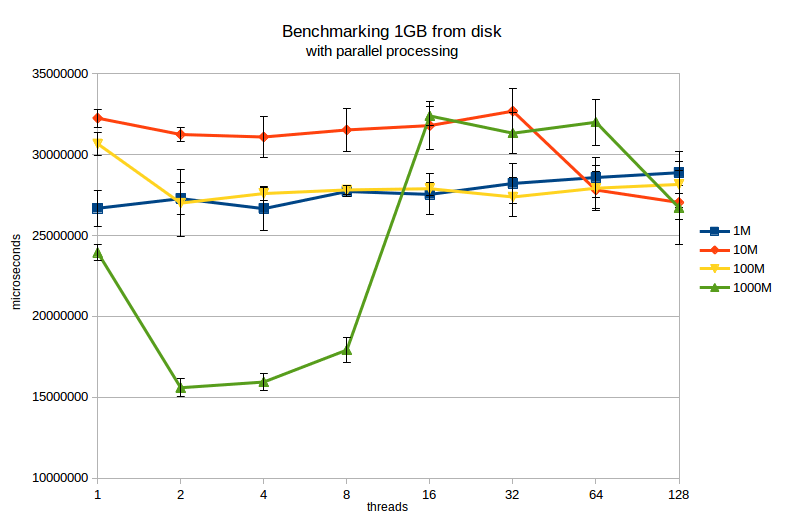
\includegraphics[scale=0.7]{../test_results/disk_par.png}
  	\caption{These are the results from running the benchmarking method on a 1GB data from a file stream, with varying amounts of available memory, from 1 megabyte to 1 gigabyte. Processing of the data was done in parallel. The standard deviation resembles the standard deviation from the disk-benchmarking and lies from 1\% to 8\%.}
	\label{figure:disk-par}
	\end{adjustwidth}
\end{figure}

% Disk Sequential
\begin{figure}
	\begin{adjustwidth}{-0.5in}{-0.5in}
    \centering
     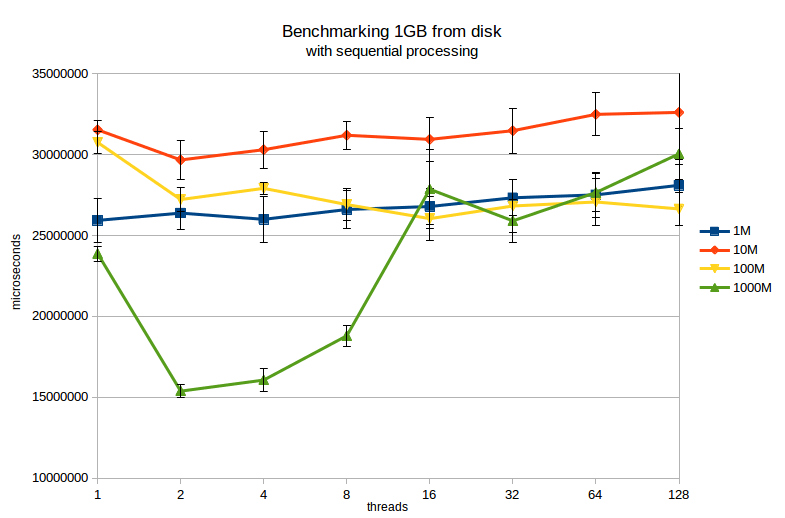
\includegraphics[scale=0.7]{../test_results/disk_seq.png}
  	\caption{These are the results from running the benchmarking method on a 1GB data from a file stream, with varying amounts of available memory, from 1 megabyte to 1 gigabyte. Processing of the data was done sequentially. The standard deviation resembles the standard deviation from the disk-benchmarking and lies from 1\% to 8\%.}
	\label{figure:disk-seq}
	\end{adjustwidth}
\end{figure}


\subsubsection{From memory}
The results from running the framework on streams of data that are already loaded into memory can be seen in \autoref{figure:mem-par} and in \autoref{figure:mem-seq}. The first one shows the results from running the system with parallel processing, where the second exhibits sequential processing. This is the ideal case, where we have a fast input stream, and we have a somewhat large amount of processing power available.\\

The practical timings in \autoref{table:io-test} shows that copying 1GB of memory takes approximately 0.2 seconds, this will be done twice in the benchmarking. First, when copying data to the worker buffers, and then to the output buffer. Further, the processing itself takes around 4.8 seconds. In total, that sums up to 5.2 seconds, if it were to be done sequentially.\\

The results shows that when we can perform sequential processing, the buffer-size does not make much of a difference. \autoref{figure:mem-par} clearly has very identical results for all four sizes of memory. With sequential processing, however, using the most memory clearly makes the framework faster. Larger buffers results in more processing, before switching threads, which in turn results in less overall locking and unlocking. The sequential processing manages to perform the benchmarks in approximately 4.8 seconds. This shows that the I/O has been hidden completely, and only the processing itself takes time. The parallel processing performs the benchmarking in approximately 1.6 seconds, effectively making it approximately 3.5 times faster thant the sequential processing. There is some inherent overhead from multithreading, which is why we can't achieve a 4 times speed-up with 4 cores.\\

The results also shows that with 1 thread, the timings match with performing the calculations in sequence. \autoref{figure:mem-seq} shows that with smaller amounts of memory, the locking becomes more expensive, with multiple threads. With 1M memory and 16 threads, there is a speed-up from 8 threads. The same tendency can be seen with 10M from 64 threads to 128 threads. This behaviour is hard to explain, and I have no apparent explanation. However, with plenty of memory, the sequential system performs best at around 8 threads. 


% Memory Parallel
\begin{figure}
	\begin{adjustwidth}{-0.5in}{-0.5in}
    \centering
     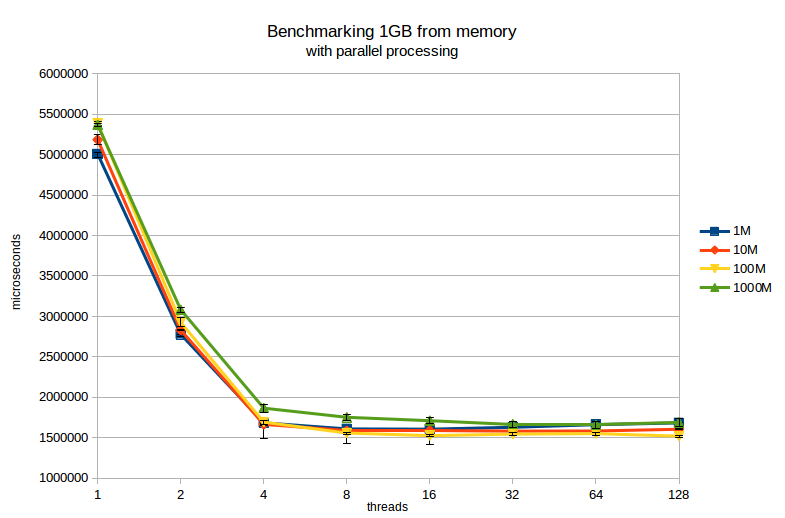
\includegraphics[scale=0.7]{../test_results/mem_par.png}
  	\caption{These are the results from running the benchmarking method on a 1GB data from main memory, with varying amounts of available memory, from 1 megabyte to 1 gigabyte. Processing of the data was done in parallel. The standard deviation resembles the standard deviation from the memory-benchmarking and lies from 1\% to 2\%.}
	\label{figure:mem-par}
	\end{adjustwidth}
\end{figure}

% Memory Sequential
\begin{figure}
	\begin{adjustwidth}{-0.5in}{-0.5in}
    \centering
     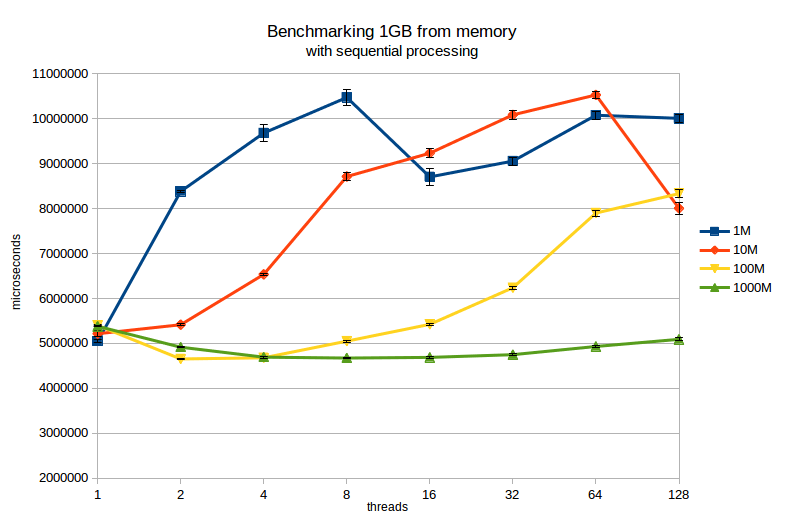
\includegraphics[scale=0.7]{../test_results/mem_seq.png}
  	\caption{These are the results from running the benchmarking method on a 1GB data from main memory, with varying amounts of available memory, from 1 megabyte to 1 gigabyte. Processing of the data was done sequentially. standard deviation resembles the standard deviation from the memory-benchmarking and lies from 1\% to 2\%.}
	\label{figure:mem-seq}
	\end{adjustwidth}
\end{figure}


\newpage
\section{Conclusion}
The \nbuf framework has been built with one main purpose. It should allow users with less experience in writing multithreaded applications to perform optimal and parallel I/O. This entails two different criteria. 

The first criteria depends on whether the framework really exhibits optimal I/O. The second criteria depends on whether the task of abstracting away the concurrency has created an interface that requires less multithreading experience to use.


\subsection{Performance}
Benchmarking the \nbuf framework has been done with a method that finds minimum and maximum values, and calculates an average value. This is a very light computation, and as such leaves most of the execution time of the framework to performing I/O. This is a good thing, because it lets us see directly, how the speed of the I/O resources affects the performance of the framework.\\

When working with a slow stream, the framework benefits from having a large amount of memory. Further, having more threads than there are hardware threads for, only reduces the efficiency. 

When using a slow hard disk drive, the sequential operation takes approximately 18.2 seconds, where the optimal configuration of the framework only takes approximately 15.1 seconds. The practical limit is approximately 13.4 seconds. This is independent of whether we perform sequential or parallel execution.\\

When working with a fast stream, the framework exhibits different behaviours when performing parallel processing and sequential processing. With sequential processing, having a large amount of memory helps. With parallel processing, the amount of memory doesn't make a large difference. In both cases, the optimal amount of threads matches with the amount of hardware threads. 

The the benchmarking task can be done sequentially in approximately 5.2 seconds, and the framework performs the benchmarking task in approximately 1.6 seconds. This is a factor 3.5 speed-up, which aligns with the 4 hardware cores on the system at hand.\\

To sum up, both with slow and fast I/O streams, speed-ups were achieved as expected. The highest throughput was obtained when having a fast stream, and parallel processing. When working with a slow stream, allocating extra memory gives a higher throughput. Using more threads than the hardware supports never gives higher throughput.


\subsection{Usefulness}
Producing on the \nbuf framework has resulted in a C++11 library that can be included by people with less experience with multi threaded applications. The library has been proven to increase performance whenever data is too large to fit in main memory, or when a small memory footprint is desired and larger amounts of data needs to be processed.

The framework gives access to native threading on most *NIX, while exposing an interface where no locks or synchronization has to be handled. The user of the library still has to know to what extend he can parallelize the task at hand, so that the task is solved correctly. This does require some amount of knowledge about how concurrency works.\\

Concurrency is inherently hard, and the framework performs correct concurrency. Users who decide to include this library will be able to perform tasks with efficient and parallel I/O, without having to debug for race conditions. This was the intention, and the framework solves the problem.\\

The framework does not yet support the queue mechanics, which is necessary for computational tasks which require more synchronization. This limitation decreases the usefulness of the system. Implementing such queue mechanic can be done rather easily, and therefore this is \textit{not a big problem}. The design has already been laid out.\\

The \nbuf framework is already available for people to work with through GitHub\footnote{The library is available on http://github.com/ath88/nbuf.}, and I expect to submit it to Boost\footnote{Boost is a repository for peer-reviewed C++ libraries. It can be found at http://www.boost.org.} if the code reaches maturity levels beyond this master's thesis.


\newpage
\section{Future Work}
The thesis work has been concluded, but there are still some missing features in the \nbuf framework, and some interesting topics to explored. 

\subsection{Missing features}
The framework misses complete support for sequential processing and in-order output. It can be implemented in the current framework, as described previously.


\subsection{Further experimentation}
While the experimentation clearly shows the effectiveness of the \nbuf framework, the experiment results also shows some odd behaviour which is not directly explainable, without more experimentation. This requires more time constructing test cases, and possibly multiple hardware setups.

Figuring out how the framework reacts in different environment can easily be a project in itself. The settings that could be varied in new experiments could be;

\begin{itemize}
\item \textbf{Different memory footprints} - Currently only 1MB, 10MB, 100MB and 1000MB were tested. I would suggest trying with a \textit{power of two}-range instead of the tenth power. This will hopefully give a more gradient view of how the framework behaves.
\item \textbf{Other disk setups} - Testing with more advanced disk set-ups would be interesting. It could be SSDs, raid configurations or network file systems.
\item \textbf{Other data sizes} - In this project I only ever tested with 1GB of data. It was a balanced amount of data which could still fit in local memory for string streams, and didn't take too long to complete the experiments. With more time, larger files could be used. This could also help strain the operating systems output buffers.
\end{itemize}


\subsection{I/O Throttling}
When large buffers are used, it takes some time before the first worker gets to processing. This will, at some point, result in lower performance than necessary. If the first thread reading would only fill a fraction of its buffer, it could start processing a lot quicker, and in turn, the entire task could be finished earlier, since more latency would be hidden.\\

A method could be to let threads fill up 10\%, then 20\%, then 40\%, then 80\% and finally 100\% for each reading operation. This will allow the threads to start processing quicker. If plenty of computation power is available, then this will result in a faster overall runtime-


\subsection{Logging and Error handling}
If an error happens in the \nbuf framework, an exception is thrown, and it is up to the user to handle it. There are some exceptions which could be handled by the framework, and the framework could in turn react by correcting, or throwing a different exception.\\

When including a third-party library, it is nice to have some kind of output, either on \textit{stdout} or \textit{stderr}, or to a stream, to be able to figure out what happens, or for debugging purposes. Currently, no such mechanism is available, and the developer has to insert debugging statements directly into the library.


\subsection{Use C++11/C++15 Features}
The current library doesn't use many of the newer features from C++11. Using smart pointers and modern allocators would help deallocating memory, when it is no longer needed. This will decrease 


\newpage
\bibliographystyle{abbrv}
\bibliography{bib}

\end{document}